\documentclass[12pt,a4paper]{report}

\usepackage{graphicx} % Ajouté pour l'inclusion des images
\usepackage{float} % Ajouté pour l'option [H] dans les figures




\begin{document}




% ----------------------
% PAGE DE GARDE
% ----------------------
\begin{titlepage}
    \centering
    \vspace*{2cm}
    {\Huge \textbf{Rapport de Stage} \par}
    \vspace{1.5cm}
    {\LARGE Développement d’un logiciel du chiffrage\par}
    \vspace{0.5cm}
    {\Large \textbf{eco-pilot} \par}
    \vspace{2cm}
    
\includegraphics[width=0.4\textwidth]{logo.png}\par % Mets ton logo ici
    \vfill
    \begin{flushright}
        \textbf{Stagiaire :} Mayar Briki \\
        \textbf{Encadrant académique :} Nom Prénom \\
        \textbf{Encadrant professionnel :} Nom Prénom \\
        \textbf{Date :} \today
    \end{flushright}
\end{titlepage}


% ----------------------
% INTRODUCTION
% ----------------------
\chapter{Introduction}
Durant mon stage de deux mois, j’ai eu l’opportunité de découvrir et de participer à des projets liés à la gestion de projets et à la gestion de budgets à travers un logiciel de chiffrage. Ce stage m’a permis de comprendre l’importance de l’organisation, du suivi des coûts et de l’optimisation des ressources pour assurer le succès des projets, tout en développant mes compétences pratiques dans un environnement professionnel. \textbf{eco-pilote}.  

% ----------------------
% ENTREPRISE
% ----------------------
\chapter{Présentation de l’entreprise}
Décrire l’entreprise d’accueil, ses activités principales et son rôle dans le projet.  

% ----------------------
% PROJET
% ----------------------
\chapter{Présentation générale du projet eco-pilote}
\section{Contexte et objectifs}
\section{Utilisateurs cibles}
\section{Fonctionnalités principales}

% ----------------------
% CAHIER DES CHARGES
% ----------------------
\chapter{Cahier des charges}
\section{Besoins fonctionnels}
\section{Besoins techniques}
\section{Contraintes}

% ----------------------
% TECHNOLOGIES
% ----------------------
\chapter{Étude et choix technologiques}
Présentation du choix de la stack \textbf{MERN (MongoDB, Express, React, Node.js)} et justification.  

% ----------------------
% CONCEPTION
% ----------------------
\chapter{Conception du projet}
\section{Architecture de l’application}
Inclure un schéma de l’architecture MERN.  

\section{Diagrammes UML}

\begin{figure}[H]
    \centering
    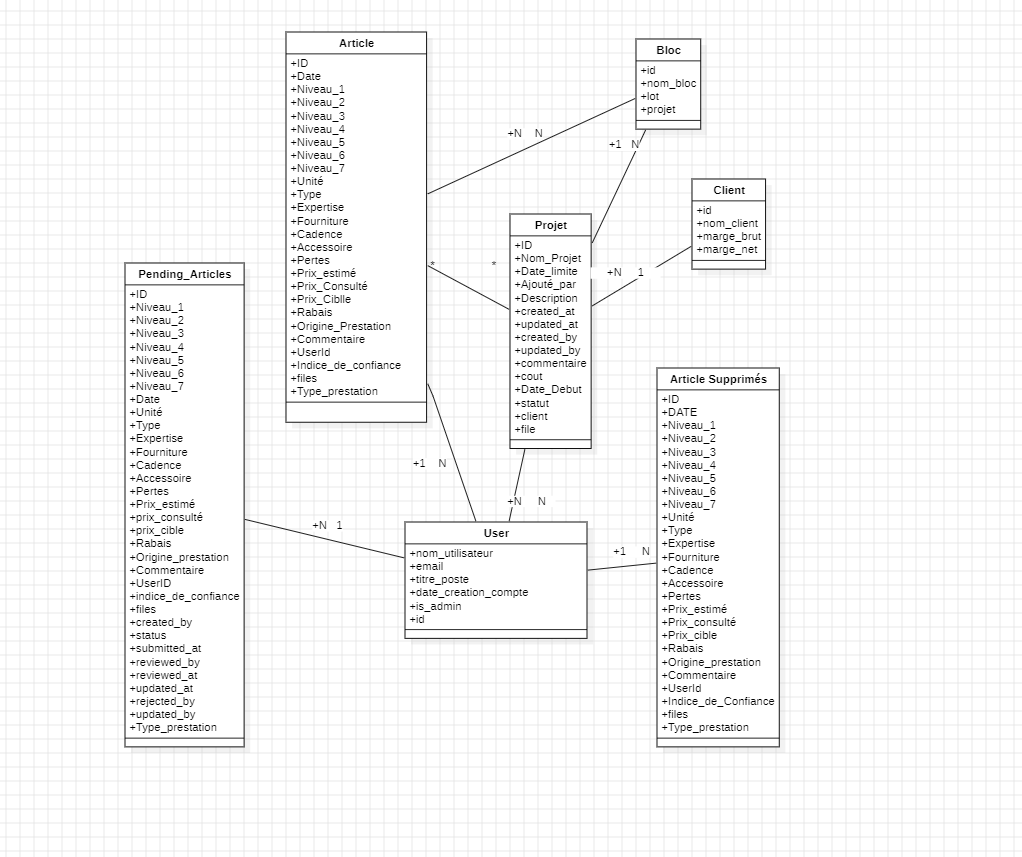
\includegraphics[width=0.5\linewidth]{image.png}
    \caption{Enter Caption}
    \label{fig:placeholder}
\end{figure}

\section{Modèle de la base de données}

% ----------------------
% IMPLÉMENTATION
% ----------------------
\chapter{Implémentation}
\section{Backend (Node.js + Express)}
\section{Frontend (React)}
\section{Base de données (MongoDB)}
\section{Sécurité et authentification (JWT, hashage)}
\section{Tests et validation}

% ----------------------
% DÉPLOIEMENT
% ----------------------
\chapter{Déploiement}
\section{Environnement de développement}
\section{Environnement de production}
\section{Gestion de versions (Git/GitHub)}
\section{CI/CD (si applicable)}

% ----------------------
% RÉSULTATS
% ----------------------
\chapter{Résultats obtenus}
Inclure captures d’écran de l’application (ex. page de connexion, tableau de bord).  

% ----------------------
% DIFFICULTÉS ET SOLUTIONS
% ----------------------
\chapter{Difficultés rencontrées et solutions}
Lister les problèmes techniques et organisationnels rencontrés ainsi que leurs solutions.  

% ----------------------
% PERSPECTIVES
% ----------------------
\chapter{Perspectives d’amélioration}
Améliorations techniques et fonctionnelles possibles.  

% ----------------------
% CONCLUSION
% ----------------------
\chapter{Conclusion}
Bilan global du stage, apports professionnels et personnels.  

% ----------------------
% ANNEXES
% ----------------------
\appendix
\chapter{Annexes}
\section{Extraits de code}
\section{Documentation API}
\section{Diagrammes complets}

% ----------------------
% BIBLIOGRAPHIE
% ----------------------
\begin{thebibliography}{9}
\bibitem{mern} Documentation officielle MERN : \url{https://www.mongodb.com/mern-stack}
\bibitem{react} Documentation React : \url{https://react.dev}
\bibitem{node} Documentation Node.js : \url{https://nodejs.org}
\end{thebibliography}

\end{document}


\section{Introduction}


\end{document}
